\subsection{Model training, validation and testing metrics functions}
procedure similar to mamo
Each will undertake the training, but the testing performed on the other to two to capture the overall system quality
Each model will go through the same proedure of testing and verification.
To start, model will be fitted on the training set of input windows for a single selected driving profile.
After each set, a validation on the similar cell at ambient temperature will be performed to get initial model performance.
The validation set is creaed from unseen data to report the acuracy of the training process only.
The training will be performed until predefined loss function achieves accuracy of bellow 2,4\% or achieve maximum possible accuracy without overfitting.
The learning steps will not be affected by the overfitting process and each failure will be preloaded with previos succesfully trained model and repeat training several times.
%
Testing perform against 2 cycles of each unsued driving profiles using one of the available embedded devices, capable for Machine Learning.
The intension was to verefy that model will be capable to be used at low power devices and still meet necessary performance requirenments.
%
So called cross-valudation mechanisim, the profile will be switched to another and perform exactly the same training, validation and testing steps.
Each result is summarised into a table and reported based on metrics valuues.

Based on the progressive error degradation, a final iteration for the discussion will be based on a lowest training and validation error.
After, the successfull model will be taken through entire unseen dataset to calculate overall accuracy against entire remaining sets.
Following plot demonstrates how multi-processing unit testing process is performed for all 3 driving profiles over single model. 

%
Test procedure performed on 2 cycles of each profiles but at different temperature to asses how perseprive model is to capture average and high temperature at which accumulator may end up.
%
% IF
\ifthenelse {\boolean{thesis}}
%
% THEN
{
\mbox{Figure~\ref{fig:device_compute}} demonstrates the paralysation mechanism for a single model, where flops and the total number of parameters are determined using the script in Appendix~\ref{app:flops}.
}
{
\mbox{Figure~\ref{fig:device_compute}} demonstrates the paralysation mechanism for a single model.% \begin{table*}[htbp]
    %     \renewcommand{\arraystretch}{1.3}
    %     \caption{Accuracy result summary - part 2.}
    %     \centering
    %     \label{tab:acc-results2}
    % \resizebox{\linewidth}{!}{
    % \begin{tabular}{ c c c c c c c }
    %     \hline\hline \\[-3mm]
    %     Model \# & Training  & Testing & Charge or Disharge & MSE(\%) & RMSE(\%) & $R^{2}$(\%) \\
    %     \hline
    %      & DST  & \makecell{DST\\US06\\FUDS} & Both 
    %                     & \makecell{5.89*\\5.46*\\7.61*} & \makecell{8.87*\\7.84*\\10.64*} & \makecell{90.91*\\92.68*\\86.45*} \\
    %     \#4%Jiao \textit{et al.}~\cite{jiao_gru-rnn_2020} 
    %      & US06 & \makecell{US06\\DST\\FUDS} & Discharge 
    %                     & \makecell{6.39*\\7.23*\\8.78*} & \makecell{8.35*\\9.68*\\12.33*} & \makecell{91.61*\\88.86*\\81.48*} \\
    %      & FUDS & \makecell{FUDS\\DST\\US06} & Discharge 
    %                     & \makecell{12.83*\\12.64*\\8.73*} & \makecell{16.02*\\15.68*\\11.71*} & \makecell{67.99*\\71.58*\\83.82*} \\
    %     \hline
    %      & DST  & \makecell{DST\\US06\\FUDS} & Both 
    %                     & \makecell{1.94\\2.60\\2.60} & \makecell{2.87\\3.64\\3.64} & \makecell{99.06\\98.42\\98.44} \\
    %      \#5%Javid \textit{et al.}~\cite{javid_adaptive_2020} 
    %      & US06 & \makecell{US06\\DST\\FUDS} & Both 
    %                     & \makecell{4.04\\5.42\\4.38} & \makecell{5.39\\7.02\\6.01} & \makecell{96.56\\94.37\\95.75} \\
    %      & FUDS & \makecell{FUDS\\DST\\US06} & Both 
    %                     & \makecell{2.13\\4.98\\2.17} & \makecell{3.28\\6.75\\3.34} & \makecell{98.73\\94.80\\98.68} \\
    %     \hline
    %      & DST  & \makecell{DST\\US06\\FUDS} & Both
    %                     & \makecell{6.06\\6.22\\6.16} & \makecell{8.09\\8.29\\8.21} & \makecell{92.38\\91.99\\92.20} \\
    %     \#6%Zhang \textit{et al.}~\cite{zhang_deep_2020} 
    %      & US06 & \makecell{US06\\DST\\FUDS} & Both 
    %                     & \makecell{5.85\\5.96\\5.98} & \makecell{7.30\\7.42\\7.72} & \makecell{93.76\\93.72\\93.52} \\
    %      & FUDS & \makecell{FUDS\\DST\\US06} & Both 
    %                     & \makecell{3.09\\6.40\\3.13} & \makecell{4.59\\8.25\\4.65} & \makecell{97.52\\92.24\\97.46} \\
    %     \hline\hline
    % \end{tabular}
    % }
    % \end{table*}
    
    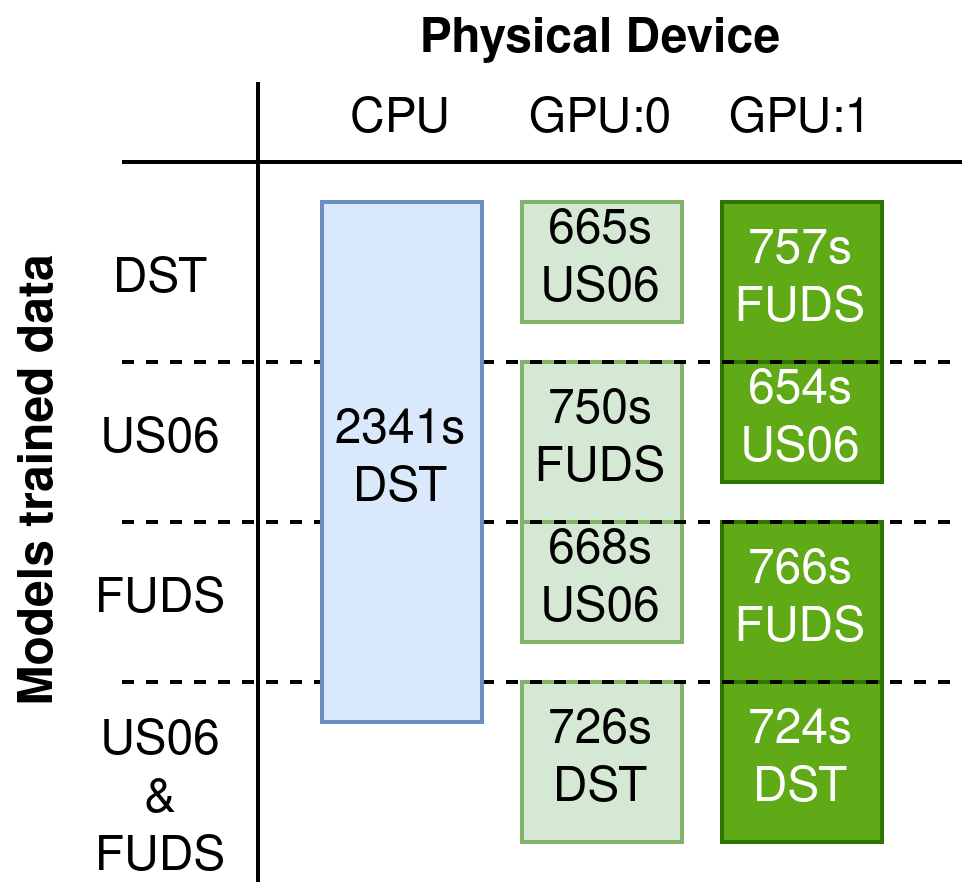
\includegraphics[width=\columnwidth]{II_Body/images/Accuracy_Compute.png}
    % \includesvg[width=\linewidth]{II_Body/images/Accuracy_Compute_10.svg}
    \caption{Accuracy computation using a single model trained on different proflies separately. The timing examples were taken from Model \#5 computation process.}
    \label{fig:device_compute}
\end{figure}


%
%
% \subsubsection{Losses}~\label{subsub:losses}
\begin{figure}[ht]
    \centering
    \includesvg[width=\columnwidth]{II_Body/images/plot-example.svg}
    \caption{Accuracy plot demonstration.}
    \label{fig:plot_demo}
\end{figure}
\mbox{Table~\ref{tab:losses}} summarises the loss functions, which has been applied to each tested model.
Some equations were extracted directly from papers; others were written based on their definition and internal library implementation.
The goal of the loss function is to calculate the error between model prediction and the actual value.
The efficiencies and impact of each equation are hard to determine and are not the investigation's goal.
The purpose of the table is only to provide the implementation references, which has been assumed during the programming of each published article based model.
\begin{table*}[htbp]
    \renewcommand{\arraystretch}{1.3}
    \caption{Model's loss functions}
    \centering
    \label{tab:losses}
    \resizebox{\linewidth}{!}{
    \begin{tabular}{ l l l c }
        \hline\hline \\[-3mm]
        Function Name & Method used in & Source articles & Equation \\ 
        \hline
        Absolute Error & & Song \textit{et al.}~\cite{song_lithium-ion_2018} & $|SoC_t-\hat{SoC_t}|$ \\
        \hline
        -- &\#1 \#4 & \makecell[l]{Chemal \textit{et al.}\cite{Chemali2017},\\Jiao \textit{et al.}~\cite{jiao_gru-rnn_2020}} & $\sum\limits^N_{t=0} \frac{1}{2} (SoC_t-\hat{SoC_t})^2$ \\
        \hline
        \makecell[l]{Mean Average\\ Percentage Error} &\#3 & Mamo \textit{et al.}~\cite{mamo_long_2020} & $\frac{100}{N}\sum\limits^N_{t=0}|\frac{SoC_t-\hat{SoC_t}}{SoC_t}|$ \\
        \hline
        -- &\#2 & Xiao \textit{et al.}~\cite{xiao_accurate_2019} & $\frac{\sum\limits^N_{t=1}(SoC_t-\hat{SoC_t})^2}{N}$ \\
        \hline
        \makecell[l]{Mean Average\\ Squared Error} &\#5 \#6 & \makecell[l]{Javid \textit{et al.}~\cite{javid_adaptive_2020},\\Zhang \textit{et al.}~\cite{zhang_deep_2020}} & $\sum\limits^N_{t=0} \sqrt{\frac{1}{n} (SoC_t-\hat{SoC_t})^2}$ \\
        \hline\hline
    \end{tabular}
    }
\end{table*}

% $ L = \sum\limits^N_{t=0} \frac{1}{2} (SoC_t-\hat{SoC_t})^2$ ~\cite{Chemali2017},~\cite{jiao_gru-rnn_2020} \\
% $ L = \sum\limits^N_{t=0} \sqrt{\frac{1}{n} (SoC_t-\hat{SoC_t})^2}$ ~\cite{javid_adaptive_2020}~\cite{zhang_deep_2020} \\
% $ L = (\sum\limits^N_{t=1}(SoC_t-\hat{SoC_t})^2)N$~\cite{xiao_accurate_2019} \\
% $ L = |SoC_t-\hat{SoC_t}|$ \\
% $ L = \frac{100}{N}\sum\limits^N_{t=0}|\frac{SoC_t-\hat{SoC_t}}{SoC_t}|$~\cite{mamo_long_2020} \\

% \ebd{table}
% $MAE = \frac{1}{N}\sum\limits^N_{t=1} |SoC_t-\hat{SoC_t}|$ \\
% $MAPE = \frac{100}{N}\sum\limits^N_{t=1}|\frac{SoC_t-\hat{SoC_t}}{SoC_t}|$ \\
% $RMSE = \sqrt{\frac{1}{N}\sum\limits^N_{t=1}(SoC_t-\hat{SoC_t})^2}$ \\
% $R^2 = 1-\frac{\sum\limits^N_{t=1}(SoC_t-\hat{SoC_t})^2}
%               {\sum\limits^N_{t=1}(SoC_t-M_{SoC})^2}$ - $M_{SoC}$ is the mean SoC \\
% $Error = \frac{SoC_t-\hat{SoC_5}}{SoC_t}$ - Not decided yet
% \subsubsection{Callbacks}
% For stateless model, the method for reseting a State of model has been derived with Callback function of:
% Another Algorithm. \\
% \begin{lstlisting}[language=Python]
% class ResetCallback(tf.keras.callbacks.Callback):
%     reset_steps : int = 500
%     i_counter   : int = 0
%     def __init__(self):
%         self.i_counter = 0

%     def on_batch_begin(self, batch, logs=None):
%         if (self.i_counter % self.reset_steps) == 0:
%             self.model.reset_states()
%             self.i_counter = 0
%         self.i_counter += 1
% \end{lstlisting}
% \begin{enumerate}
%     \item Checkpoint saving only the best one based on smalest rmse
%     \item Tensorboard tmp folder
%     \item Early stopping is applyable
%     \item Procedure of training epoch by epoch or algorithm for offline and online.
% \end{enumerate}
% \subsubsection{Callbacks}
% \begin{itemize}
%     \item Checkpoint \\
%     \item Tensorboard \\
%     \item nanTerminate \\    
% \end{itemize}
% \subsubsection{Training and validation Loop??}
% \begin{itemize}
%     \item validation over what data? - single cycle \\
% \end{itemize}
% \subsubsection{Testing procedures??}
% \begin{itemize}
%     \item Converting model to the TF-Lite usage for TPU processor \\
%     \item 2 profiles - two cycle test \\
% \end{itemize}

%
%
% \subsubsection{Metrics}
% \textcolor{red}{Generally, Losses start form 0, metrics from 1. Articles which did overwise were assumed to be mistaken.}
% \textcolor{red}{Similar to loses and reasons why we have chosen those as out criterias.} \\
Metrics functions act as user evaluation criteria to assess the performance of the trained model during both fitting and validation processes.
Although some papers relied on different evaluation criteria, for this research, metrics were unified with several equations from \mbox{Table~\ref{tab:metrics}}.
Thus, the same criteria will be used for the final comparison between models' efficiency in the results section.
\begin{table}[htbp]
    \renewcommand{\arraystretch}{1.3}
    \caption{Model's metrics functions}
    \centering
    \label{tab:metrics}
    \resizebox{\columnwidth}{!}{
    \begin{tabular}{l c}
        \hline\hline \\[-3mm]
        Function Name & Equation \\ 
        \hline
        \makecell[l]{Mean Average\\ Error} &  $\frac{1}{N}\sum\limits^N_{t=1} |SoC_t-\hat{SoC_t}|$ \\
        % \hline
        % Mean Average Percentage Error & $\frac{100}{N}\sum\limits^N_{t=1}|\frac{SoC_t-\hat{SoC_t}}{SoC_t}|$ \\
        \hline
        \makecell[l]{Root Mean\\ Square Error} & $ \sqrt{\frac{1}{N}\sum\limits^N_{t=1} \left(SoC_t-\hat{SoC_t} \right)^2}$ \\
        \hline
        \makecell[l]{$R^2$ : $M_{SoC}$ is\\ the mean SoC} & $1-\frac{\sum\limits^N_{t=1}(SoC_t-\hat{SoC_t})^2}
                {\sum\limits^N_{t=1}(SoC_t-M_{SoC})^2}$ \\
        \hline\hline
        % Error : Not decided if useful yet & $ \frac{SoC_t-\hat{SoC_5}}{SoC_t}$
    \end{tabular}
    }
\end{table}

